\documentclass[sigconf]{acmart}

\usepackage{subfigure}
\usepackage{enumitem}

% Here are two macros for comments.
\newcommand {\nred}[1]{{\color{red}\sf{[#1]}}}
\newcommand {\ngreen}[1]{{\color{green}\sf{[#1]}}}
\newcommand {\ncyan}[1]{{\color{cyan}\sf{[#1]}}}
\newcommand {\michael}[1]{{\color{red}\sf{[michael: #1]}}}
\newcommand {\charles}[1]{{\color{blue}\sf{[charles: #1]}}}
\newcommand {\serena}[1]{{\color{orange}\sf{[charles: #1]}}}

%%
%% \BibTeX command to typeset BibTeX logo in the docs
\AtBeginDocument{%
  \providecommand\BibTeX{{%
    \normalfont B\kern-0.5em{\scshape i\kern-0.25em b}\kern-0.8em\TeX}}}

%% Rights management information.  This information is sent to you
%% when you complete the rights form.  These commands have SAMPLE
%% values in them; it is your responsibility as an author to replace
%% the commands and values with those provided to you when you
%% complete the rights form.
%%MM: NO FOR SUBMISSION%% \setcopyright{acmcopyright}
%%MM: NO FOR SUBMISSION%% \copyrightyear{2XXX}
%%MM: NO FOR SUBMISSION%% \acmYear{2XXX}
%%MM: NO FOR SUBMISSION%% \acmDOI{10.1145/1122445.1122XXX}

%% These commands are for a PROCEEDINGS abstract or paper.
%%MM: NO FOR SUBMISSION%% \acmConference[Woodstock '18]{Woodstock '18: ACM Symposium on Neural
%%MM: NO FOR SUBMISSION%%   Gaze Detection}{June 03--05, 2018}{Woodstock, NY}
%%MM: NO FOR SUBMISSION%% \acmBooktitle{Woodstock '18: ACM Symposium on Neural Gaze Detection,
%%MM: NO FOR SUBMISSION%%   June 03--05, 2018, Woodstock, NY}
%%MM: NO FOR SUBMISSION%% \acmPrice{15.00}
%%MM: NO FOR SUBMISSION%% \acmISBN{978-1-4503-XXXX-X/18/06}


%%
%% Submission ID.
%% Use this when submitting an article to a sponsored event. You'll
%% receive a unique submission ID from the organizers
%% of the event, and this ID should be used as the parameter to this command.
%%\acmSubmissionID{123-A56-BU3}

%%
%% The majority of ACM publications use numbered citations and
%% references.  The command \citestyle{authoryear} switches to the
%% "author year" style.
%%
%% If you are preparing content for an event
%% sponsored by ACM SIGGRAPH, you must use the "author year" style of
%% citations and references.
%% Uncommenting
%% the next command will enable that style.
%%\citestyle{acmauthoryear}

%%
%% end of the preamble, start of the body of the document source.
\begin{document}

%%
%% The "title" command has an optional parameter,
%% allowing the author to define a "short title" to be used in page headers.
\title{%
Predicting trends in the quality of state-of-the-art neural networks without access to training or testing data
}

%%
%% The "author" command and its associated commands are used to define
%% the authors and their affiliations.
%% Of note is the shared affiliation of the first two authors, and the
%% "authornote" and "authornotemark" commands
%% used to denote shared contribution to the research.

%%MM: NO FOR SUBMISSION%% \author{Charles H. Martin}
%%MM: NO FOR SUBMISSION%% \affiliation{%
%%MM: NO FOR SUBMISSION%%   \institution{Calculation Consulting}
%%MM: NO FOR SUBMISSION%%   \streetaddress{8 Locksley Ave, 6B}
%%MM: NO FOR SUBMISSION%%   \city{San Francisco, CA 94122}
%%MM: NO FOR SUBMISSION%%   \country{USA}}
%%MM: NO FOR SUBMISSION%% \email{charles@CalculationConsulting.com}
%%MM: NO FOR SUBMISSION%% 
%%MM: NO FOR SUBMISSION%% \author{Tongsu (Serena) Peng}
%%MM: NO FOR SUBMISSION%% \affiliation{%
%%MM: NO FOR SUBMISSION%%   \institution{XXX Same as me}
%%MM: NO FOR SUBMISSION%%   \streetaddress{XXX}
%%MM: NO FOR SUBMISSION%%   \city{Irvine, CA, 92612}
%%MM: NO FOR SUBMISSION%%   \country{USA}}
%%MM: NO FOR SUBMISSION%% \email{serenapeng7@gmail.com}
%%MM: NO FOR SUBMISSION%% 
%%MM: NO FOR SUBMISSION%% \author{Michael W. Mahoney}
%%MM: NO FOR SUBMISSION%% \affiliation{%
%%MM: NO FOR SUBMISSION%%   \institution{ICSI and Department of Statistics, University of California at Berkeley}
%%MM: NO FOR SUBMISSION%%   \streetaddress{XXX}
%%MM: NO FOR SUBMISSION%%   \city{Berkeley, CA 94720}
%%MM: NO FOR SUBMISSION%%   \country{USA}}
%%MM: NO FOR SUBMISSION%% \email{mmahoney@stat.berkeley.edu}

%%
%% By default, the full list of authors will be used in the page
%% headers. Often, this list is too long, and will overlap
%% other information printed in the page headers. This command allows
%% the author to define a more concise list
%% of authors' names for this purpose.
%\renewcommand{\shortauthors}{Trovato and Tobin, et al.}

%%
%% The abstract is a short summary of the work to be presented in the
%% article.
\begin{abstract}
Abstract

\end{abstract}

%%
%% The code below is generated by the tool at http://dl.acm.org/ccs.cfm.
%% Please copy and paste the code instead of the example below.
%%
%%MM: NO FOR SUBMISSION%% \begin{CCSXML}
%%MM: NO FOR SUBMISSION%% <ccs2012>
%%MM: NO FOR SUBMISSION%%  <concept>
%%MM: NO FOR SUBMISSION%%   <concept_id>10010520.10010553.10010562</concept_id>
%%MM: NO FOR SUBMISSION%%   <concept_desc>Computer systems organization~Embedded systems</concept_desc>
%%MM: NO FOR SUBMISSION%%   <concept_significance>500</concept_significance>
%%MM: NO FOR SUBMISSION%%  </concept>
%%MM: NO FOR SUBMISSION%%  <concept>
%%MM: NO FOR SUBMISSION%%   <concept_id>10010520.10010575.10010755</concept_id>
%%MM: NO FOR SUBMISSION%%   <concept_desc>Computer systems organization~Redundancy</concept_desc>
%%MM: NO FOR SUBMISSION%%   <concept_significance>300</concept_significance>
%%MM: NO FOR SUBMISSION%%  </concept>
%%MM: NO FOR SUBMISSION%%  <concept>
%%MM: NO FOR SUBMISSION%%   <concept_id>10010520.10010553.10010554</concept_id>
%%MM: NO FOR SUBMISSION%%   <concept_desc>Computer systems organization~Robotics</concept_desc>
%%MM: NO FOR SUBMISSION%%   <concept_significance>100</concept_significance>
%%MM: NO FOR SUBMISSION%%  </concept>
%%MM: NO FOR SUBMISSION%%  <concept>
%%MM: NO FOR SUBMISSION%%   <concept_id>10003033.10003083.10003095</concept_id>
%%MM: NO FOR SUBMISSION%%   <concept_desc>Networks~Network reliability</concept_desc>
%%MM: NO FOR SUBMISSION%%   <concept_significance>100</concept_significance>
%%MM: NO FOR SUBMISSION%%  </concept>
%%MM: NO FOR SUBMISSION%% </ccs2012>
%%MM: NO FOR SUBMISSION%% \end{CCSXML}
%%MM: NO FOR SUBMISSION%% 
%%MM: NO FOR SUBMISSION%% \ccsdesc[500]{Computer systems organization~Embedded systems}
%%MM: NO FOR SUBMISSION%% \ccsdesc[300]{Computer systems organization~Redundancy}
%%MM: NO FOR SUBMISSION%% \ccsdesc{Computer systems organization~Robotics}
%%MM: NO FOR SUBMISSION%% \ccsdesc[100]{Networks~Network reliability}

%%
%% Keywords. The author(s) should pick words that accurately describe
%% the work being presented. Separate the keywords with commas.
%%MM: NO FOR SUBMISSION%% \keywords{XXX, datasets, neural networks, gaze detection, text tagging}

%% A "teaser" image appears between the author and affiliation
%% information and the body of the document, and typically spans the
%% page.
%\begin{teaserfigure}
%  \includegraphics[width=\textwidth]{sampleteaser}
%  \caption{Seattle Mariners at Spring Training, 2010.}
%  \Description{Enjoying the baseball game from the third-base
%  seats. Ichiro Suzuki preparing to bat.}
%  \label{fig:teaser}
%\end{teaserfigure}

%%
%% This command processes the author and affiliation and title
%% information and builds the first part of the formatted document.
\maketitle

%KDD% \vspace{-1mm}
\section{Introduction}
\label{sxn:intro}

Over the past decade, Deep Neural Networks (DNNs) have proven remarkably effective on a wide range of 
computer vision (CV), natual language processing (NLP), and other domains.  
Moreover, larger and deeper DNN models, with hundreds to thousands of layers, perform tasks
seemingly impossible just a few years ago.  
For example, the CV architecture ResNet has been successfuly trained with over 1000 layers,
showing excellent generqlization performance on a wide range of data sets (CIFAR10, CIFAR100, SVHN, ImagaeNet, etc.
Most recently, openAI released the NLP Language model GPT3, which has been trained on nearly a half trillion words,
using 175 billion parameters, and achieving state-of-the-art (SOTA) performance on several NLP
benchmarks.  

The incredible size and depth of these models poses a new and deep theoretical challenges.
[blah blah blah]
Discuss Energy Landscape and  ruggedly convexity


\nred{What has been done before}

\nred{Cross Sections}
We do have some insight into how the Energy Landscape behaves by visualizing 2-dimensional
cross-sections of small models during training, such as ResNet25.
Maybe can run ourselves ?

\nred{Analysis of the Hessian}
Not really informative.  Hessian only provides local information.


\nred{Empirical Generalization Metrics}
Norm-based metrics such as WeightWatcher
Correlated with generalization / test accuracy.
Best metric is based on power law / heavy tailed.
Not explicitly data dependent



\nred{What needs to be done}
Cross-Section is not a generalization metric, is not global

Importance of unsupervised metrics: self training


In order to characterize the Energy Landscape, traditional approaches attempt to count
the number of local minima (i.e the complexity).  And while this is well for theoretical
analysis (such as spin glass theory, random matric theory, etc), numerically this
is quite hard.  Especially for the massive production size DNNs in use today.

Here, we suggest an new, alternative approach--to study the Empirical Spectral Density (ESD)
of the data-dependent Jacobian, which is readily calculated with a single epoch of Backprop
using any off-the-shelf toolkit such as TensorFlow, PyTorch, etc. 

Similar to the weightwatcher studies..

Show picture:  compare relatively random / flat vs  a deeply funneled convex Landscape ESDs

random:  real world data, randomly labeled 




Here is a summary of our main results:
\begin{itemize}
\item

\item

\item 

\end{itemize}


\paragraph{Funneled Enegy Landscapes}
\nred{where to put this ?}
\begin{figure}[h]
\begin{center}
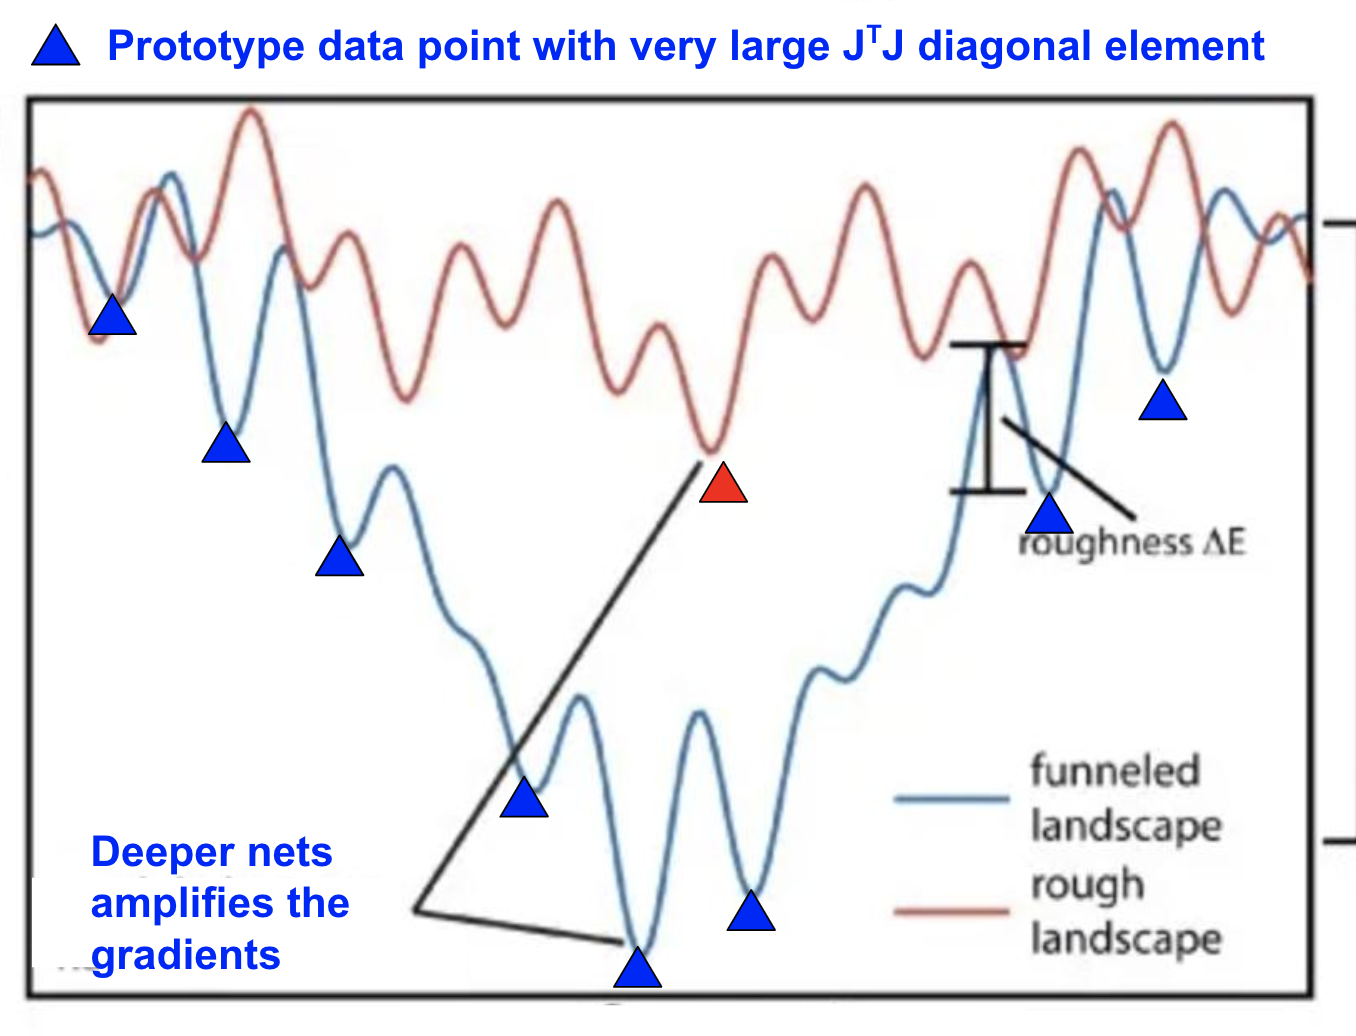
\includegraphics[scale=0.2]{img/funnel.png}
\end{center}
\caption{Sample figure caption.}
\label{fig:funnel}
\end{figure}




\paragraph{Organization of this paper.}




%KDD% \vspace{-1mm}
\section{Conclusion}
\label{sxn:conc}
%\vspace{-1mm}

CONCLUSION



%%
%% The acknowledgments section is defined using the "acks" environment
%% (and NOT an unnumbered section). This ensures the proper
%% identification of the section in the article metadata, and the
%% consistent spelling of the heading.

%%MM: NO FOR SUBMISSION%% \begin{acks}
%%MM: NO FOR SUBMISSION%% MWM would like to acknowledge ARO, DARPA, NSF, and ONR for providing partial support of this work.
%%MM: NO FOR SUBMISSION%% We would also like to thank Amir Khosrowshahi and colleagues at Intel for helpful discussion regarding the Group Regularization distillation technique.
%%MM: NO FOR SUBMISSION%% \end{acks}

\vspace{-2mm}

%%
%% The next two lines define the bibliography style to be used, and
%% the bibliography file.
\bibliographystyle{ACM-Reference-Format}
%\bibliography{gen_gap}
\bibliography{dnns}
%\bibliography{dnns,gen_gap}

\newpage
\appendix
\section{Appendix}
\label{sxn:appendix}

In this appendix, we provide more details on several issues that are important for the reproducibility of our results.



\end{document}

